% Straight up stealing preamble from Eli Holmes 
%%%%%%%%%%%%%%%%%%%%%%%%%%%%%%%%%%%%%%START PREAMBLE THAT IS THE SAME FOR ALL EXAMPLES
\documentclass{article}

%Required: You must have these
\usepackage{Sweave}
\usepackage{graphicx}
\usepackage{tabularx}
\usepackage{hyperref}
\usepackage{natbib}
\usepackage{pdflscape}
\usepackage{array}
\usepackage{gensymb}
%\usepackage[backend=bibtex]{biblatex}
%Strongly recommended
  %put your figures in one place
%\SweaveOpts{prefix.string=figures/, eps=FALSE} 
%you'll want these for pretty captioning
\usepackage[small]{caption}

\setkeys{Gin}{width=0.8\textwidth}  %make the figs 50 perc textwidth
\setlength{\captionmargin}{30pt}
\setlength{\abovecaptionskip}{10pt}
\setlength{\belowcaptionskip}{10pt}
% manual for caption  http://www.dd.chalmers.se/latex/Docs/PDF/caption.pdf

%Optional: I like to muck with my margins and spacing in ways that LaTeX frowns on
%Here's how to do that
 \topmargin -1.5cm        
 \oddsidemargin -0.04cm   
 \evensidemargin -0.04cm  % same as oddsidemargin but for left-hand pages
 \textwidth 16.59cm
 \textheight 21.94cm 
 %\pagestyle{empty}       % Uncomment if don't want page numbers
 \parskip 7.2pt           % sets spacing between paragraphs
 %\renewcommand{\baselinestretch}{1.5} 	% Uncomment for 1.5 spacing between lines
\parindent 0pt% sets leading space for paragraphs
\usepackage{setspace}
%\doublespacing

%Optional: I like fancy headers
%\usepackage{fancyhdr}
%\pagestyle{fancy}
%\fancyhead[LO]{How do climate change experiments actually change climate}
%\fancyhead[RO]{2016}
 
%%%%%%%%%%%%%%%%%%%%%%%%%%%%%%%%%%%%%%END PREAMBLE THAT IS THE SAME FOR ALL EXAMPLES

%Start of the document
\begin{document}

%\SweaveOpts{concordance=TRUE}
 \bibliographystyle{/Users/aileneettinger/citations/Bibtex/styles/amnat.bst}
\title{Spatial and temporal shifts in photoperiod with climate change} % perspective paper for OSPREE analyses

\author{A.K. Ettinger, D. Buonaiuto, C. Chamberlain, I. Morales-Castilla, E. Wolkovich}
%\date{\today}%do we need to also add any of the following: D. Flynn, T. Savas, J. Samaha, E. Forrestel? 
\maketitle  %put the fancy title on
%\tableofcontents      %add a table of contents
%\clearpage
%%%%%%%%%%%%%%%%%%%%%%%%%%%%%%%%%%%%%%%%%%%%%%%%%%%

%%%%%%%%%%%%%%%%%%%%%%%%%%%%%%%%%%%%%%%%%%%%%%%%%%%

\section*{Summary}
Recent warming temperatures have brought about temporal shifts in biological activity, such as spring budburst and fall senescence, as well as spatial shifts in species' distributions. These temporal and spatial shifts are expected to continue with future warming, and will alter the photoperiod experienced by diverse species. To date, photoperiod has not been a focus of climate change forecasting, despite the fact that photoperiod responses are common (observed in 26/31 or 84\% of studies that manipulated photoperiod in woody plant species). We argue that temporal shifts are expected to have a major impact on experienced photoperiod, so additional testing of the importance of photoperiod to phenology and adding it to forecasts of biological shifts should be major goals. We find that, though many experiments impose photoperiod treatments well outside current and expected future conditions, there is a substantial resource of studies with relevant treatments that could be used to forecast implications of photoperiod shifts with climate change. We highlight outstanding questions that are in need of additional research and modelling approaches to improve predictions of when, where, and how much photoperiod is likely to affect future phenology.

\section*{Introduction}
\par  Photoperiod is a critical cue for plants, signalling changes to their activities, such as photosynthesis, growth, reproduction, dormancy, and senescence \citep[e.g.,][]{Howe:1996,lagercrantz2009}. Photoperiod is used by plants to synchronize their activities with seasonal climatic changes \citep[e.g.,][]{Hsu:2011,Singh:2017,Basler:2012} because it is consistent across years, especially compared to other seasonal cues such as temperature and precipition \citep{saikkonen2012}. For example, relying on photoperiod, rather than temperature alone, may prevent plants from leafing out during ``false spring" events \citep[unusually warm periods during winter that are followed by a return of cold temperatures][] {Gu2008})). 
\par We know that photoperiod is an important cue for spring budburst phenology, largely through growth chamber experiments.  These experiments often manipulate photoperiod in combination with temperature to address basic questions about how these two environmental drivers act as biological cues. Air temperature has a dual role in regulating phenology: chilling, the prolonged exposure to cold temperatures after growth cessation in the fall, that is required to break dormancy within the bud; and forcing, prolonged exposure to warm temperatures, that is required for budburst to occur. Thus, chilling and forcing temperatures are often altered in addition to photoperiod in growth chamber experiments \citep[e.g.,][]{Campbell:1975aa,HEIDE:1977aa,Falusi:1990aa,Spann:2004aa,Laube:2014a}. Growth chamber studies have been conducted for decades, but have only recently been synthesized (cite our paper). This synthesis reveals wide variation in sensitivity to photoperiod across species and populations. 
\par Recent studies offer conflicting evidence %would prefer a different word here, as not all papers offer evidence- sometimes it is opinion/ideas based on theory...suggestions?) 
about the extent to which photoperiod may control spring phenology in a warmer world. Some studies suggest that certain species, such as late successional taxa, will be unable to track climate warming, i.e., by leafing out earlier in the spring and senescing later in the fall \citep{koerner2010b} (Any Other studies with similar ideas?). Instead, these species will increasingly become constrained by daylength, since  photoperdio sensitivity is primarily genetically controlled \citep{koerner2010b}. Other studies, however, suggest that photoperiod is unlikely to constrain responses to warming for most species \citep{zohner2016} (others?).
 

\par Perhaps because of these conflicting views, photoperiod is often not included in forecasts of biological responses to climate change even though it is known to be an important cue for platn activity \citet[but see ][]{duputie2015}. %% IMC- I'm not sure forecasts of biological responses to climate change focus on temperature. Most literature on SDMs forecasting species distributions uses a bunch of environmental variables (see http://worldclim.org/bioclim) to fit the models with subsequent problems of collinearity (but that's another topic). Perhaps we could mention, that amongst the 'usual suspect' environmental variables used to fit forecasts, photoperiod is rarely included.
The exclusion of photoperiod may be problematic because, although photoperiod itself is stable over time, the photoperiod that species \emph{experience}, as they undergo climate change-induced shifts in space and time, is likely to be much less stable. With recent warming, many species have shifted their distributions poleward and upward in elevation \citep[i.e., range shifts][]{parmesan2006,chen2011,harsch2009})), and/or shifted their activity earlier in the year \citep[i.e., phenological shifts][]{parmesan2006, wolkovich2012}. These spatial and temporal shifts will alter the photoperiod regime experienced by organisms. \par The implications of potential climate-change induced shifts in experienced photoperiod are unclear, since the magnitude of potential shifts has not been described. Shifts may be relatively minor, especially because there can be substantial year-to-year background variation in experienced photoperiod (Figure \ref{fig:greenup}). Alternatively, photoperiod may begin to constrain species responses to climate change \citep{koerner2010b}.

\par Here, we ask: 
\begin{enumerate}
\item Do results from growth chamber experiments suggest that photoperiod responses are widespread in woody plants?
\item How will climate change alter the photoperiod experienced by organisms, given observed climate change-induced biological shifts, both spatially and temporally?
\item What are the implications of altered photoperiods for biological responses to climate change?
\item Can data from growth chamber experiments altering photoperiod be applied to forecasting biological implications of climate change (i.e., do they occur at the appropriate scale)?

\end{enumerate}
\par We address these questions using a new database of plant growth chamber studies that manipulate photoperiod and temperature and measure plant responses, including budburst, flowering, and growth. We focus on woody species for because plant growth chamber experiments using woody plant material have been conducted for decades, because the importance of photoperiod versus temperature effects on phenology remain controversial in woody species, and because forecasting effects of climate change on woody plant phenology (i.e., the length of the growing season) has critical implications for global carbon cycling and feedbacks to the climate system. 

\section*{Are photoperiod responses common in woody plants?}

\par Growth chamber experiments suggest that photoperiod responses are common in woody plant species. Thirty-one of the 85 studies in the OSPREE database included two or more different photoperiod treatments. Of these, 26 (84\%) found significant photoperiod main effects or significant interactive effects with temperature (Table \ref{table:phototreats}). Main effects included responses such as growth \citep[e.g., higher growth rates with longer days ][]{Ashby:1962aa}, onset of dormancy \citep[e.g., more rapid induction of budset with shorter days][]{Howe:1995aa}, and reproduction \citep[e.g., increased flowering with longer days ][]{Heide:2012aa}. 
\par Growth chamber experiments demonstrate that, though photoperiod responses are common, they are variable (Figure \ref{fig:photocurve}). Responses to photoperiod commonly differ by species \citep[e.g.,][]{Heide:1993a,Howe:1996,Basler:2012, Basler:2014aa,zohner2016,flynn2018}. For example, with long chilling treatments some species seem insensitive to daylength (e.g.,Cat- could you add a sp or 2 from zohner), whereas others (e.g. \emph{Fagus} spp.) seem to have daylength requirements to break dormancy, even with long chilling treatments \citep{zohner2016}. %could also use heide93a for example: Long days reduced the thermal time to budburst in all flushing species except Sorbus acuparia and Rubus ideaus
Photoperiod sensitivity also varies by populations and ecotypes  \citep[e.g.,][]{Partanen:2005aa,flynn2018}. For example, photoperiod effects on budburst were  more significant for lower latitude populations of \emph{Betula pendula} and \emph{B. pubescens} \citep{Partanen:2005aa}.
\par In addition to the variation among species and populations, growth chamber experiments highlight that responses to photoperiod vary depending on the temperature. For example, more rapid advancement of budburst was observed under long versus short days with low chilling, than with high chilling \citep{Hawkins:2012}. 

\section*{How will climate change alter the photoperiod experienced by organisms?}
\par Species experience different photoperiod regimes depending on their location in space and the seasonal timing of their activity. The daylength experienced by plants on spring green-up date, for example, varies with latitude, (Figure \ref{fig:greenup}a). This is in part because of latitudinal variation in both photoperiod and green-up date, which occurrs earlier toward the equator and later toward the poles. Athough the general pattern is consistent across years (Figure \ref{fig:greenup}b), there is strong spatiotemporal variation in experienced photoperiod (Figure \ref{fig:greenup}c).% A year that results in early green-up at 35\degree, for instance, may not be an early year at 50\degree latitude (Figure \ref{fig:greenup}c).

\par Against this existing background variation, climate change is likely to cause average shifts in experienced photoperiod, as species respond to warming temperatures. Spatial shifts in species' ranges and temporal shifts in  phenology will alter the photoperiods experienced by organisms with future climate change. The magnitude of these alterations will vary depending on the organism's location and the type of shift(s) it undergoes. For example, poleward shifts in species' ranges cause organisms to experience a wider range of daylength throughout the year (Figure \ref{fig:spacetime}). Elevational shifts, on the other hand, would cause minimal changes in daylength throughout the year. 
\par To date, most of the scientific literature has focused on how spatial range shifts linked to climate change will affect photoperiod \citep{saikkonen2012} (other citations?). Shifting phenology will also alter experienced photoperiod, because of the seasonal patterns of daylength (Figure \ref{fig:spacetime}). To understand the magnitude of change in experienced photoperiod with spatial versus temporal shifts in organisms activity, we compared photoperiods across latitudes and days that differed at relevant scales, given observed shifts in  species' ranges and phenology \citep{parmesan2003,chen2011}.  
\par We found that temporal shifts are actually likely to yield bigger changes in experienced photoperiod than spatial shifts (Figure \ref{fig:spacetime}). For example, consider a tree at latitude 45\degree that completes spring budbursts, on average, around DOY 91 (April 2, when daylength is 12.8 hours). If its phenology shifts 30 days earlier over the next century \citep[][i.e., a rate of ~3 days per decade, as has been observed]{parmesan2003}, it will experience a daylength that is 1.6 hours shorter. However, if the same tree species shifts its range up in latitude 0.5\degree (i.e., 60 km over the next century,  comparable to observed rates \citep{parmesan2003, chen2011}), it will experience a daylength that differs by less than a minute on the same DOY. Importantly, growth chamber studies demonstrate that the magnitudes of daylength shifts we can expect with climate change (i.e. 1-2 hours difference in daylength with temporal shifts over the next century) are substantial enough to alter phenology(cite new table).  
\par In many cases organisms may shift both their geographic ranges and their phenology simulataneously. In addition, photoperiod sensitivity, or the degree to which phenology is controlled by daylength, can vary with latitude \citep{Howe:1996,saikkonen2012,Partanen:2005aa,Vihera-Aarnio:2006aa,Caffarra:2011b,gauzere2017}, perhaps because of population-level differences in sensitivity. With future climate change, it is unclear how these complications will affect the photoperiod experienced by organisms and if these shifts in photoperiod will have important implications for biological responses. 
% IMC - I like Cat's suggestion. Somehow we should note that there is a ('circular'?) feedback between phenology-photoperiod, so that phenology shifts alter experienced photoperiod, which in turn affects phenology (as well as other biological features, e.g. behavior).

\section*{What are the implications of altered photoperiods for biological responses to climate change?}
\par Daylength plays a role in controling critical plant functions, including vegetative growth, cell elongation, budburst, and flowering \citep{Linkosalo:2006aa,erwin1998,sidaway2010, Hsu:2011,Heide:2011aa,Ashby:1962aa,Heide:2012aa,mimura2007}. Climate change-induced shifts in photoperiod are therefore likely to alter these functions. The direction and magnitude of such alterations will vary, however, because of variation in photoperiod sensitivity, and because photoperiod often interacts with other environmental drivers, such as temperature, to affect phenology. 

\par %Phenology is generally controlled by photoperiod and temperature. For example, the timing of spring budburst in woody plants is controlled by interactions between chilling, forcing, and daylength \citep{flynn2018,Heide:2008aa, zohner2016}. 
Over the past century, budburst has shifted earlier in diverse woody species (CITES), a pattern that, to date, can be largely explained by warming temperatures. Photoperiod may eventually become a limiting factor, however, constraining the ability of species to respond to additional warming \citep{koerner2010b,vitasse2013, Morin:2010aa,Nienstaedt:1966aa}. Interactions between photoperiod and temperature may therefore result in muted phenological shifts, compared to what would be expected based on temperature change alone \citep{wareing1956,mimura2007,koerner2010b}. If photoperiod does becomes limiting, phenology may shift abruptly, not gradually, because photoperiod sensitivity is thought to be a theshold response (Box 1). 
\par A challenge in understanding biological responses to shifts in photoperiod is the wide range of sensitivity observed across species \citep{Sanz-Perez:2009aa, zohner2016,flynn2018}, populations \citep{tanino2010}, and ecotypes\citep{Howe:1995aa}. Some of this variation is likely due to underlying genetic differences, because photoperiod responses are thought to be under strong genetic control \cite{bradshaw1995,weih2004,keller2011}. This variation may also be explained by different combinations of ambient temperature and photoperiod, because temperature cues can override photoperiod requirements under certain conditions \citep [e.g., during growth cessation][] {tanino2010}. In such cases, climate change induced phenological shifts may occur at different rates than past shifts with warming. 
\par Indeed, future rates of phenological shifts are unlikely be a straightforward extrapolation from current and past rates, in most cases. Predicting future shifts is further complicated by the spatial and temporal variation in experienced photoperiod, and by varying sensitivity to photoperiod across species and populations.  Methods for incoporating photoperiod into forecasting future phenology and other biological responses would therefore be incredibly useful.
\section*{Future directions: outstanding questions and incorporating photoperiod into forecasting}
\par Approaches to forecasting biological responses to climate change can be grouped into two broad categories: statistical models and process-based models. %These two categories are, in reality, extreme cases at two ends of a spectrum of modelling approaches, because most statistical models have a little process (i.e., predictor variables) and most process-based models have some assumed statistical relationships.
These two modelling extremes differ in at least two ways, in terms of relating plant phenology to climate change. First, statistical models generally assume linear relationships between species' responses and environmental variables \citep[e.g., EXAMPLES][]{flynn2018}, whereas process-based models incorporate nonlinear threshold relationships as well (e.g., PhenoFit). Second, statistical models of phenology under climate change have typically ignored photoperiod, focusing instead on seasonal or annual temperature,% Or, as lizzie said: To date in statistical models many people either ignore photoperiod or they put it in in some very painful way ('we added photoperiod experienced on the day of budburst to the PEP725 data to test for the role of photoperiod') that is not well designed. 
whereas process-based models are more likely to incorporate photoperiod, along with forcing and chilling. The challenge of process-based models is that they require detailed data (e.g., daily climate data, nonlinear biological responses). Perhaps because of this challenge, statistical models remain more commonly used in climate change forecasts of biological responses (I think this is true, but need data/citation to back this up!). % Cat: Laube14 (GCB) does a binomial GLM and looks at interactions, Basler12, Basler14 and Vitasse14 (Tree Phys) all do ANOVAs - not sure this is enough evidence but we use these for Ospree.
% IMC: A suggestion for the above sentence: "The challenge of process-based models is that they are 'data-hungry' and require  data at high spatial and temporal resolutions (e.g., daily climate data, nonlinear biological responses), that are often not available for most species/ecosystems." 
\par Whether statistical or process-based approaches are used, future modelling can incorporate photoperiod by leveraging the large amount of experimental data on photoperiod responses (Figure \ref{fig:photomap}, Table \ref{table:phototreats}). Researchers can use these data to first learn if their species (or a closely related species) shows a photoperiod effect, and, ideally, how it varies by population, ecotype, or other factors. If there is evidence of a photoperiod response, daylength should be added to forecasting models (Figure \ref{fig:condiag}). Given the large change in experienced photoperiod with temporal shifts (Figure \ref{fig:spacetime}), this may be particularly important for phenology forecasting. Since spatial shifts are associated with smaller changes in experienced photoperiod, it may be less important for distribution forecasts.
That being said, species are likely to shift in \emph{both} space and time simultaneously. Thus, even though experienced photoperiod changes little as species distributions shift in space, phenology may be altered significantly, and have cascading effects on plant growth and fitness\citep{duputie2015}. %not sure this is the best citation. 
\par In many cases, experimental data can be immediately used in forecasting because experiments manipulate photoperiod at relevant scales (e.g., \citet{Basler:2014aa,Heide:2015aa}, Figures \ref{fig:photomap}, \ref{fig:fagus}, Table \ref{table:phototreats}).  The available data can inform critical non-linearities and variations across species, and/or populations (Figure \ref{fig:condiag}.  Adding photoperiod and variable responses to forecasts could fundamentally alter the future species and communities we expect, especially since plants are thought to respond to photoperiod in a threshold manner (Box 1, Figure \ref {fig:photocurve}). 

\par In other cases, attempting to incorporate photoperiod into forecasts of future phenology will higlight that there is a great need to better understand many aspects of photoperiod responses. Thus, modelling efforts may inspire additional experiments to test some of the critical predictions and assumptions that they make, and address outstanding questions in the field. Through the process of incorporating experimental data into more process-based models, it is likely that knowlege gaps will be identified. For example, many experiments manipulate photoperiod much more dramatically than will occur with climate change (Figures \ref{fig:photomap}, \ref{fig:fagus},\ref{fig:quercus}. Extrapolating these findings with models may be difficult. 
\par Additional areas of further research to improve our understanding of the effects of shifts in photoperiod with climate change include:
\begin{enumerate}
\item \underline{How does photoperiod act as a cue?} The divergent effects of photoperiod observed across studies (e.g., Figure \ref{fig:photocurve}) suggests that photoperiod interacts with other environmental drivers, such as chilling and forcing, to affect phenology and other activities. However, exactly how it interacts with temperature to break dormancy, as well as the type of response it ellicits (e.g., linear versus threshold) is not well-defined for many species.  
\item \underline{What are the causes and consequences of species- and population-level variation in photoperiod sensitivy?} For example, what traits are associated with photoperiod sensitivity and does this variation have a strong genetic component? If so, are species or populations from some locations more likely than others to be constrained by photoperiod in their responses to climte change?

\item \underline{Does incorporating photoperiod responses alter forecasting outcomes, at population, commnity, and ecosystem scales?}  Photoperiod is incorporated into foreacasts, along with other variables such as evaporative demand, and temperature, in many ecosytem models \citep [e.g. ED] []{jolly2005, medvigy2013}. The sensitivity of model outcomes to assumptions made about photoperiod and photoperiod responses should be more widely tested, e.g. in different ecosystems, and across different species and populations.
\item \underline{How much does model accuracy (process-based or statistical) improve when we include photoperiod responses and changes in photoperiod, in addition to forecasted temperature shifts?}
\item Other ideas?
\end{enumerate}


\section*{Conclusions}
Organisms may undergo large changes to the photoperiod they experience, with climate change, even if they do not shift their ranges spatially. An altered photoperiod is likely to have implications for a variety of plant responses, as well as responses in animals and other organisms, given the diverse species for which daylength affects activities \citep[e.g.,][] {taranger2003,bradshaw2006,mcallan2006,linn1996,Flynn:2018,solbakken1994}. Incorporating photoperiod into forecasting of climate change responses may improve model accuracy, and is likely to highlight additional experiments needed to improve our mechanistic understanding of photoperiod as a cue to diverse biological responses. 
\section* {Glossary}
\begin{itemize}
\item \underline{chilling}: a required amount hours or days of cold temperature, defined by a specific critical temperature (e.g., 0 \degree C- or what is most common?), that must be experienced to break dormancy

\item \underline{endodormancy}
\item \underline{ectodormancy} 
\item \underline{forcing}: required amount of hours or days above some specific critical temperatures, that must be experienced before budburst or flowering can occur.
\item \underline{external coincidence model}
\item \underline{vernalization}
\end{itemize}
\section{Box 1. How do plants interpret photoperiod? }
\par Here we focus on spring budburst responses to photoperiod. However, our understanding of how plants interpet photoperiod comes largely from studies of flowering in the model plant \emph{Arabidopsis thaliana} (citations) and budset in woody plant species \citep{Howe:1996} (add more citations). Budburst phenology in woody plants may sense photoperiod through similar pathways, though this is not known \citep{lagercrantz2009}(other citations comparing populus to arabidopsis?). 
\par Plants are thought to interpret photoperiod through a coordinated response to light in relation to the time of day. When the internal circadean rhythm coincides with an external signal (light) under certain conditions, the responses is induced \citep{lagercrantz2009}. This ``external coincidence model" has been most widely studied in \emph{Arabidopsis}, and is thought to be a relevant mechanism for photoperiod responses in diverse perennial and woody plant species as well \citep{davis2002,petterle2013,bastow2002,kobayashi2007,andres2012,Singh:2017}. (add Bunning 1936). The model proposes the existence of a circadian rhythm of light sensitivity, in which the night-phase is sensitive to light and the day-phase is insensitive to light. As days get longer in the spring, daylight illuminates the  light sensitive phase, triggering a response.%Do we want a figure of this? 


\par Other things to consider adding to this box:
\begin{enumerate}
\item what parts of the arabidopsis photoperiod sensing mechanism is maintained in populus or other woody species?
\item what part of wood plants senses light (phytochrome, particular tissues- buds)
\item talk about photoperiod as a gate keeper to other cues and responses?
\end{enumerate}


\section* {To do:}
\begin{enumerate}
\item Update table/map to fix 2 studies have a max NA and a min NA- these look reasonable so add them with an *
\item Make lines thicker/darker in Figure 2 (looks a bit washed out)
\item Work Figures 5 and 6 more explicitly into the paper
\end{enumerate}

\bibliography{/Users/aileneettinger/Documents/GitHub/ospree/refs/ospreebibplus}
\clearpage


\section* {Tables}
% latex table generated in R 3.4.2 by xtable 1.8-2 package
% Wed Dec  5 14:54:52 2018
\begin{table}[ht]
\centering
\caption{\textbf{Growth chamber experiments and their photoperiod treatments}. We note whether or not photoperiod had a significant effect (`effect' column) and compared treatments to the spatial and temporal shifts required for organisms to experiments photoperiod changes equivalent to those treatments. For shifts in space, `ER' indicates that the photoperiod treatments exceeds the change of photoperiod from moving up to 40 degrees latitudinally on June 21. For shifts in time, `ER' indicates that the range of photoperiod treatments exceeds the change in daylengths at that latitude during the entire year. `max NA' indicates that the maximum daylength treatment does not exist at that latitude; `min NA'indicates that the minimum daylength treatment does not exist at that latitude.} 
\label{table:phototreats}
\begin{tabular}{|p{0.18\textwidth}|p{0.15\textwidth}|p{0.08\textwidth}|p{0.08\textwidth}|p{0.04\textwidth}|p{0.08\textwidth}|p{0.06\textwidth}|p{0.06\textwidth}|p{0.14\textwidth}|}
  \hline
idstudy & continent & lat & long & effect & day\_range & delta & space & time \\ 
  \hline
ashby62\_exp1 & north america & 42.99 & -89.41 & Y & 8-16 & 4.00 & 18.2 & min NA (9) \\ 
  basler14\_exp1 & europe & 46.31 & 8.27 & Y & 9.2-16 & 1.00 & 6 & -22 \\ 
  caffarra11b\_exp2 & europe & 52.32 & -6.93 & Y & 10-16 & 2.00 & 7.5 & -30 \\ 
  falusi90\_exp1 & europe & 46.03 & 10.75 & N & 9-13 & 4.00 & 16 & -82 \\ 
  falusi96\_exp3 & europe & 38.27 & 15.99 & Y & 9-13 & 4.00 & 21.6 & -111 \\ 
  ghelardini10\_exp1 & europe & 43.72 & 11.37 & N & 8-16 & 8.00 & 21.9 & ER \\ 
  heide05\_exp1 & europe & 56.18 & -4.32 & Y/N & 10-24 & 14.00 & ER & ER \\ 
  heide08\_exp1 & europe & 48.40 & 11.72 & Y & 10-24 & 14.00 & ER & ER \\ 
  heide11\_exp1 & europe & 59.67 & 10.67 & N & 10-20 & 10.00 & ER & max NA (18.7) \\ 
  heide12\_exp1 & europe & 56.50 & -3.06 & Y & 10-24 & 5.00 & 8.9 & -64 \\ 
  heide15\_exp2 & europe & 56.50 & -3.06 & Y & 10-15 & 1.00 & 3.2 & -13 \\ 
  heide93\_exp1 & europe & 59.50 & 10.77 & Y & 8-24 & 16.00 & ER & ER \\ 
  heide93a\_exp1 & europe & 59.67 & 10.83 & Y & 8-24 & 16.00 & ER & ER \\ 
  heide93a\_exp3 & europe & 47.50 & 7.60 & Y & 13-16 & 1.00 & 5.7 & -18 \\ 
  howe95\_exp1 & north america & 40.55 & -124.10 & Y & 9-24 & 2.00 & 13.1 & -64 \\ 
  laube14a\_exp1 & europe & 48.40 & 11.71 & N & 8-16 & 4.00 & 14.3 & -87 \\ 
  myking95\_exp1 & europe & 56.10 & 9.15 & Y & 8-24 & 16.00 & ER & ER \\ 
  nienstaedt66\_exp1 & north america & 44.17 & -103.92 & Y & 8-20 & 12.00 & ER & ER \\ 
  okie11\_exp1 & north america & 32.12 & -83.12 & Y & 0-12 & 12.00 & ER & ER \\ 
  partanen01\_exp1 & europe & 61.93 & 26.68 & Y & 6-16 & 10.00 & ER & -105 \\ 
  partanen05\_exp1 & europe & 61.82 & 29.32 & Y & 5-20 & 5.00 & ER & -67 \\ 
  partanen98\_exp1 & europe & 60.03 & 23.05 & Y & 8.66-12 & 3.34 & 5.1 & -37 \\ 
  pettersen71\_exp1 & europe & 59.66 & 10.77 & N & 10-24 & 2.00 & 4 & -23 \\ 
  Sanz-Perez09\_exp1 & europe & 40.40 & -3.48 & Y & 10-16 & 6.00 & 23.6 & ER \\ 
  viheraaarnio06\_exp1 & europe & 60.45 & 24.93 & Y & 16-17 & 1.00 & 2.1 & -12 \\ 
  viheraaarnio06\_exp1 & europe & 67.73 & 24.93 & Y & 20-21 & 1.00 & ER & -5 \\ 
  viheraaarnio06\_exp2 & europe & 60.45 & 24.93 & Y & 15-19 & 4.00 & 5.1 & -62 \\ 
  viheraaarnio06\_exp2 & europe & 67.73 & 24.93 & Y & 22-23 & 1.00 & ER & -3 \\ 
  worrall67\_exp 3 & north america & 41.31 & -72.93 & Y & 8-16 & 8.00 & 24.3 & ER \\ 
  zohner16\_Exp1 & europe & 48.16 & 11.50 & Y & 8-16 & 8.00 & ER & ER \\ 
  hawkins12\_ &  &  &  & Y &  &  &  &  \\ 
   \hline
\end{tabular}
\end{table}\clearpage
\section* {Figures}
\begin{figure}[p]
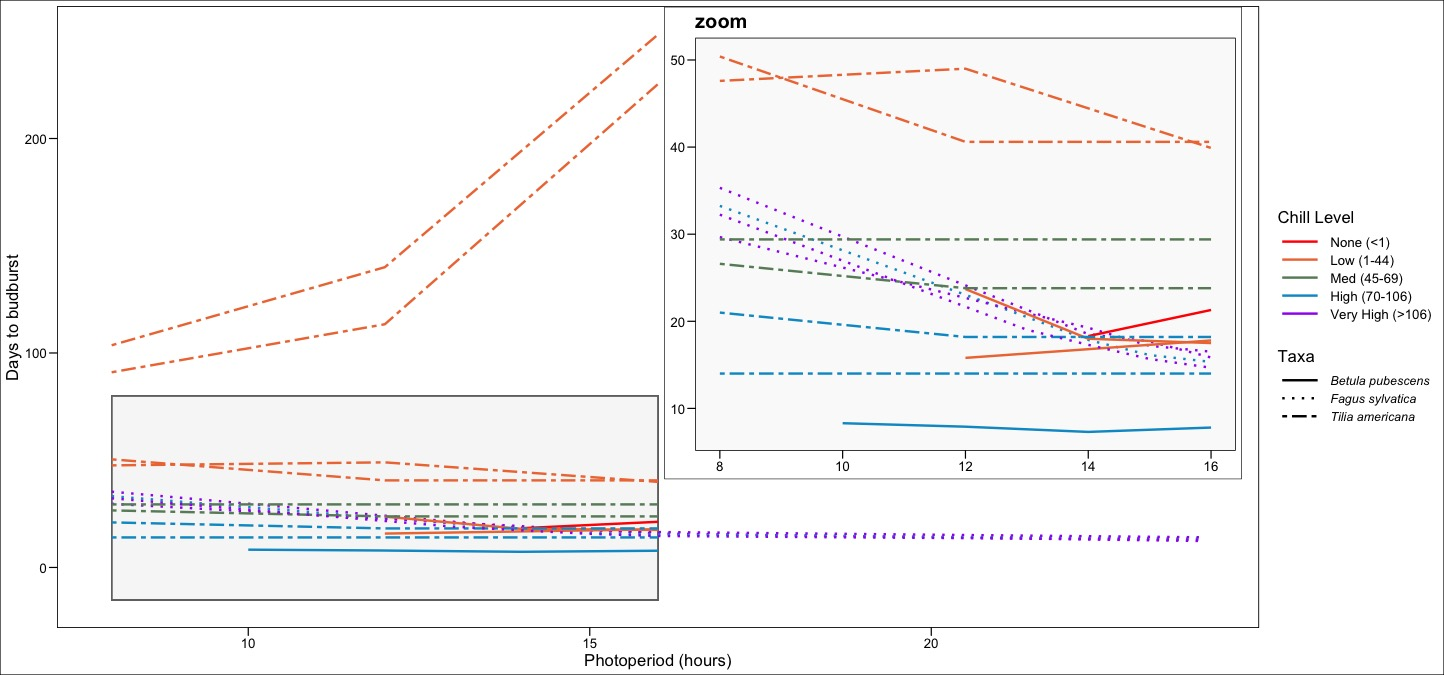
\includegraphics{/Users/aileneettinger/Documents/GitHub/ospree/analyses/photoperiod/figures/Photo_curv_FINAL.jpeg} 
\caption{\textbf{Plant responses to changes in daylength vary across species and populations, and with the amount of chilling recieved}.}
 \label{fig:photocurve}
 \end{figure}

\begin{figure}[p]
\centering
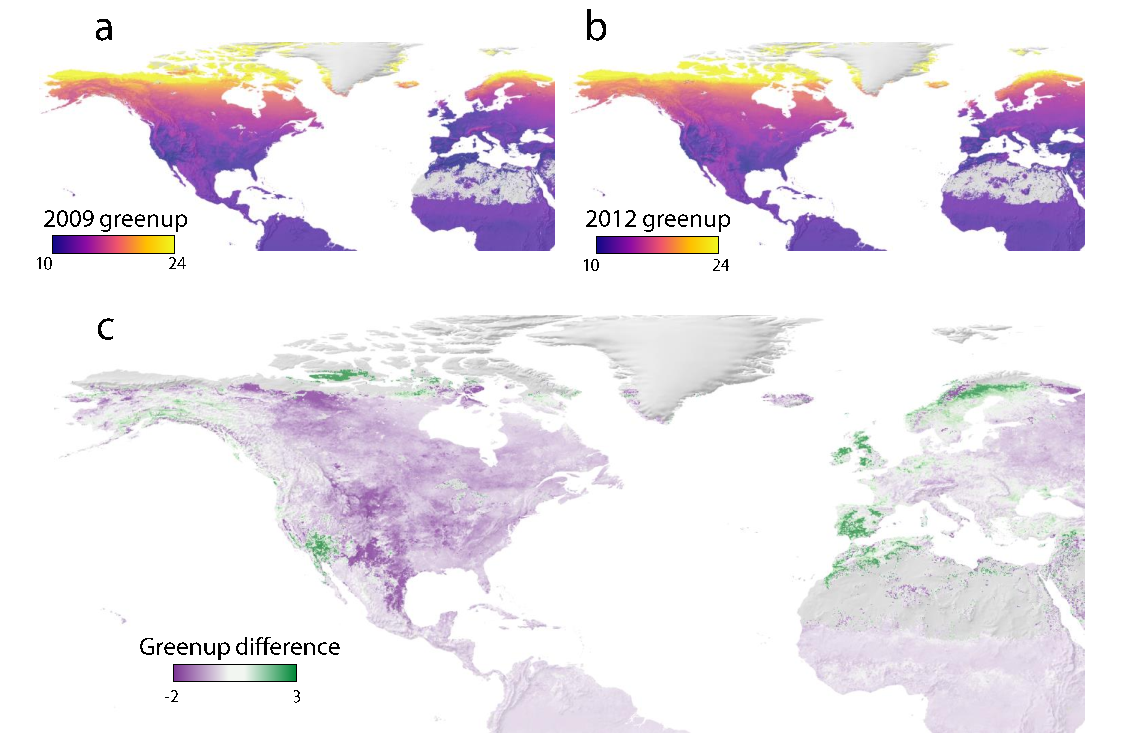
\includegraphics{/Users/aileneettinger/Documents/GitHub/ospree/docs/photoperiod/figures/Greenup_corr.pdf} %2009 greenup
\caption{\textbf{The photoperiod on the green up date (start of spring) varies over space} and among years. Hours of daylight on the date of spring green up from MODIS satilite data across North America and Europe for an average (2009, a) and  early (2012,b) North American start of spring. The differences between the years are shown in (c). }
 \label{fig:greenup}%
 \end{figure}


\begin{figure}[p]
\centering
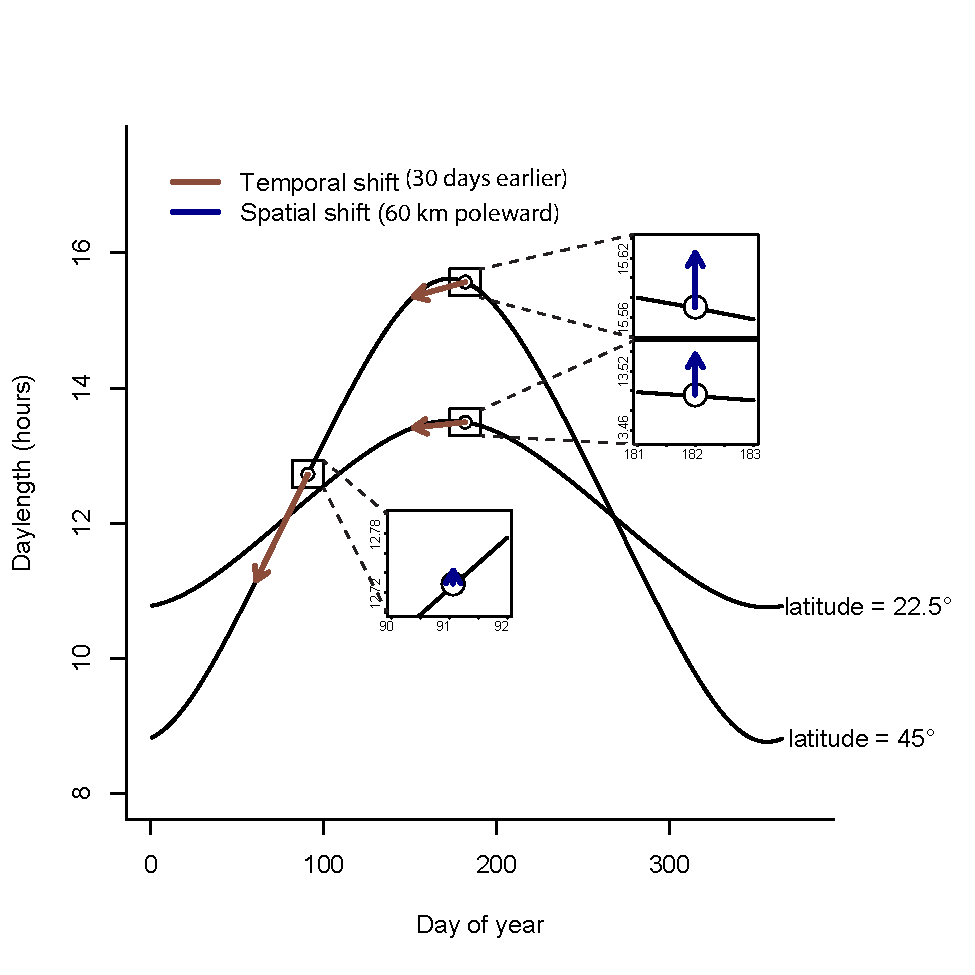
\includegraphics{/Users/aileneettinger/Documents/GitHub/ospree/analyses/photoperiod/figures/photo_spacetime_v2.pdf} %
\caption{\textbf{Photoperiod varies with latitude and throughout the year}, such that temporal shifts in activity yield larger changes in experienced photoperiod compared with spatial shifts. Here, we show this variation at two latitudes, using hypothetical rates of spatial and temporal shifts: 30 days earlier for temporal shifts, and 0.5 degrees poleward for spatial shifts. These shifts, which are similar to observed average rates \citep[e.g.,][]{parmesan2006,chen2011}, highlight the greater magnitude in daylength changes close to the equinox (e.g., DOY 91), versus close to the summer solcstice (e.g., DOY 182).}
 \label{fig:spacetime}%
 \end{figure}
 
\begin{figure}[p]
\centering
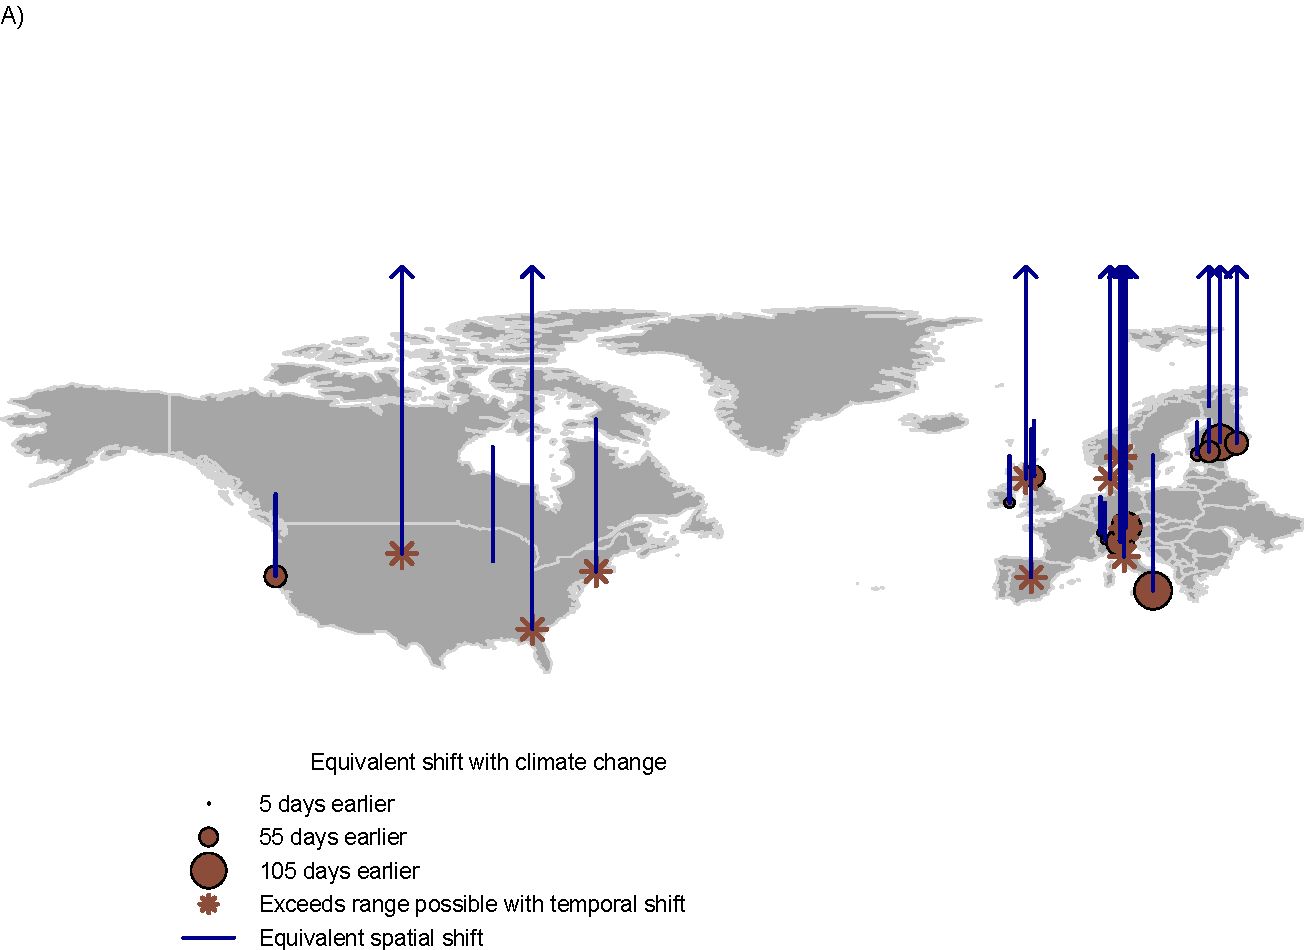
\includegraphics{/Users/aileneettinger/Documents/GitHub/ospree/analyses/photoperiod/figures/ospree_photopmap.pdf} 
\caption{\textbf{OSPREE experiments that manipulate photoperiod}, and their equivalent spatial and temporal shifts, mapped (A), and graphed (B-C). Observed rates (dashed gray lines) 16.9 kilometers per decade (or approximately 1.5 degrees in 100 years) for spatial shifts (Chen et al. 2011) and 2.3 days per decade (or 23 days in 100 years) for temporal shifts (Parmesan and Yohe 2003).}
 \label{fig:photomap}
 \end{figure}


 
 
\begin{figure}[p]
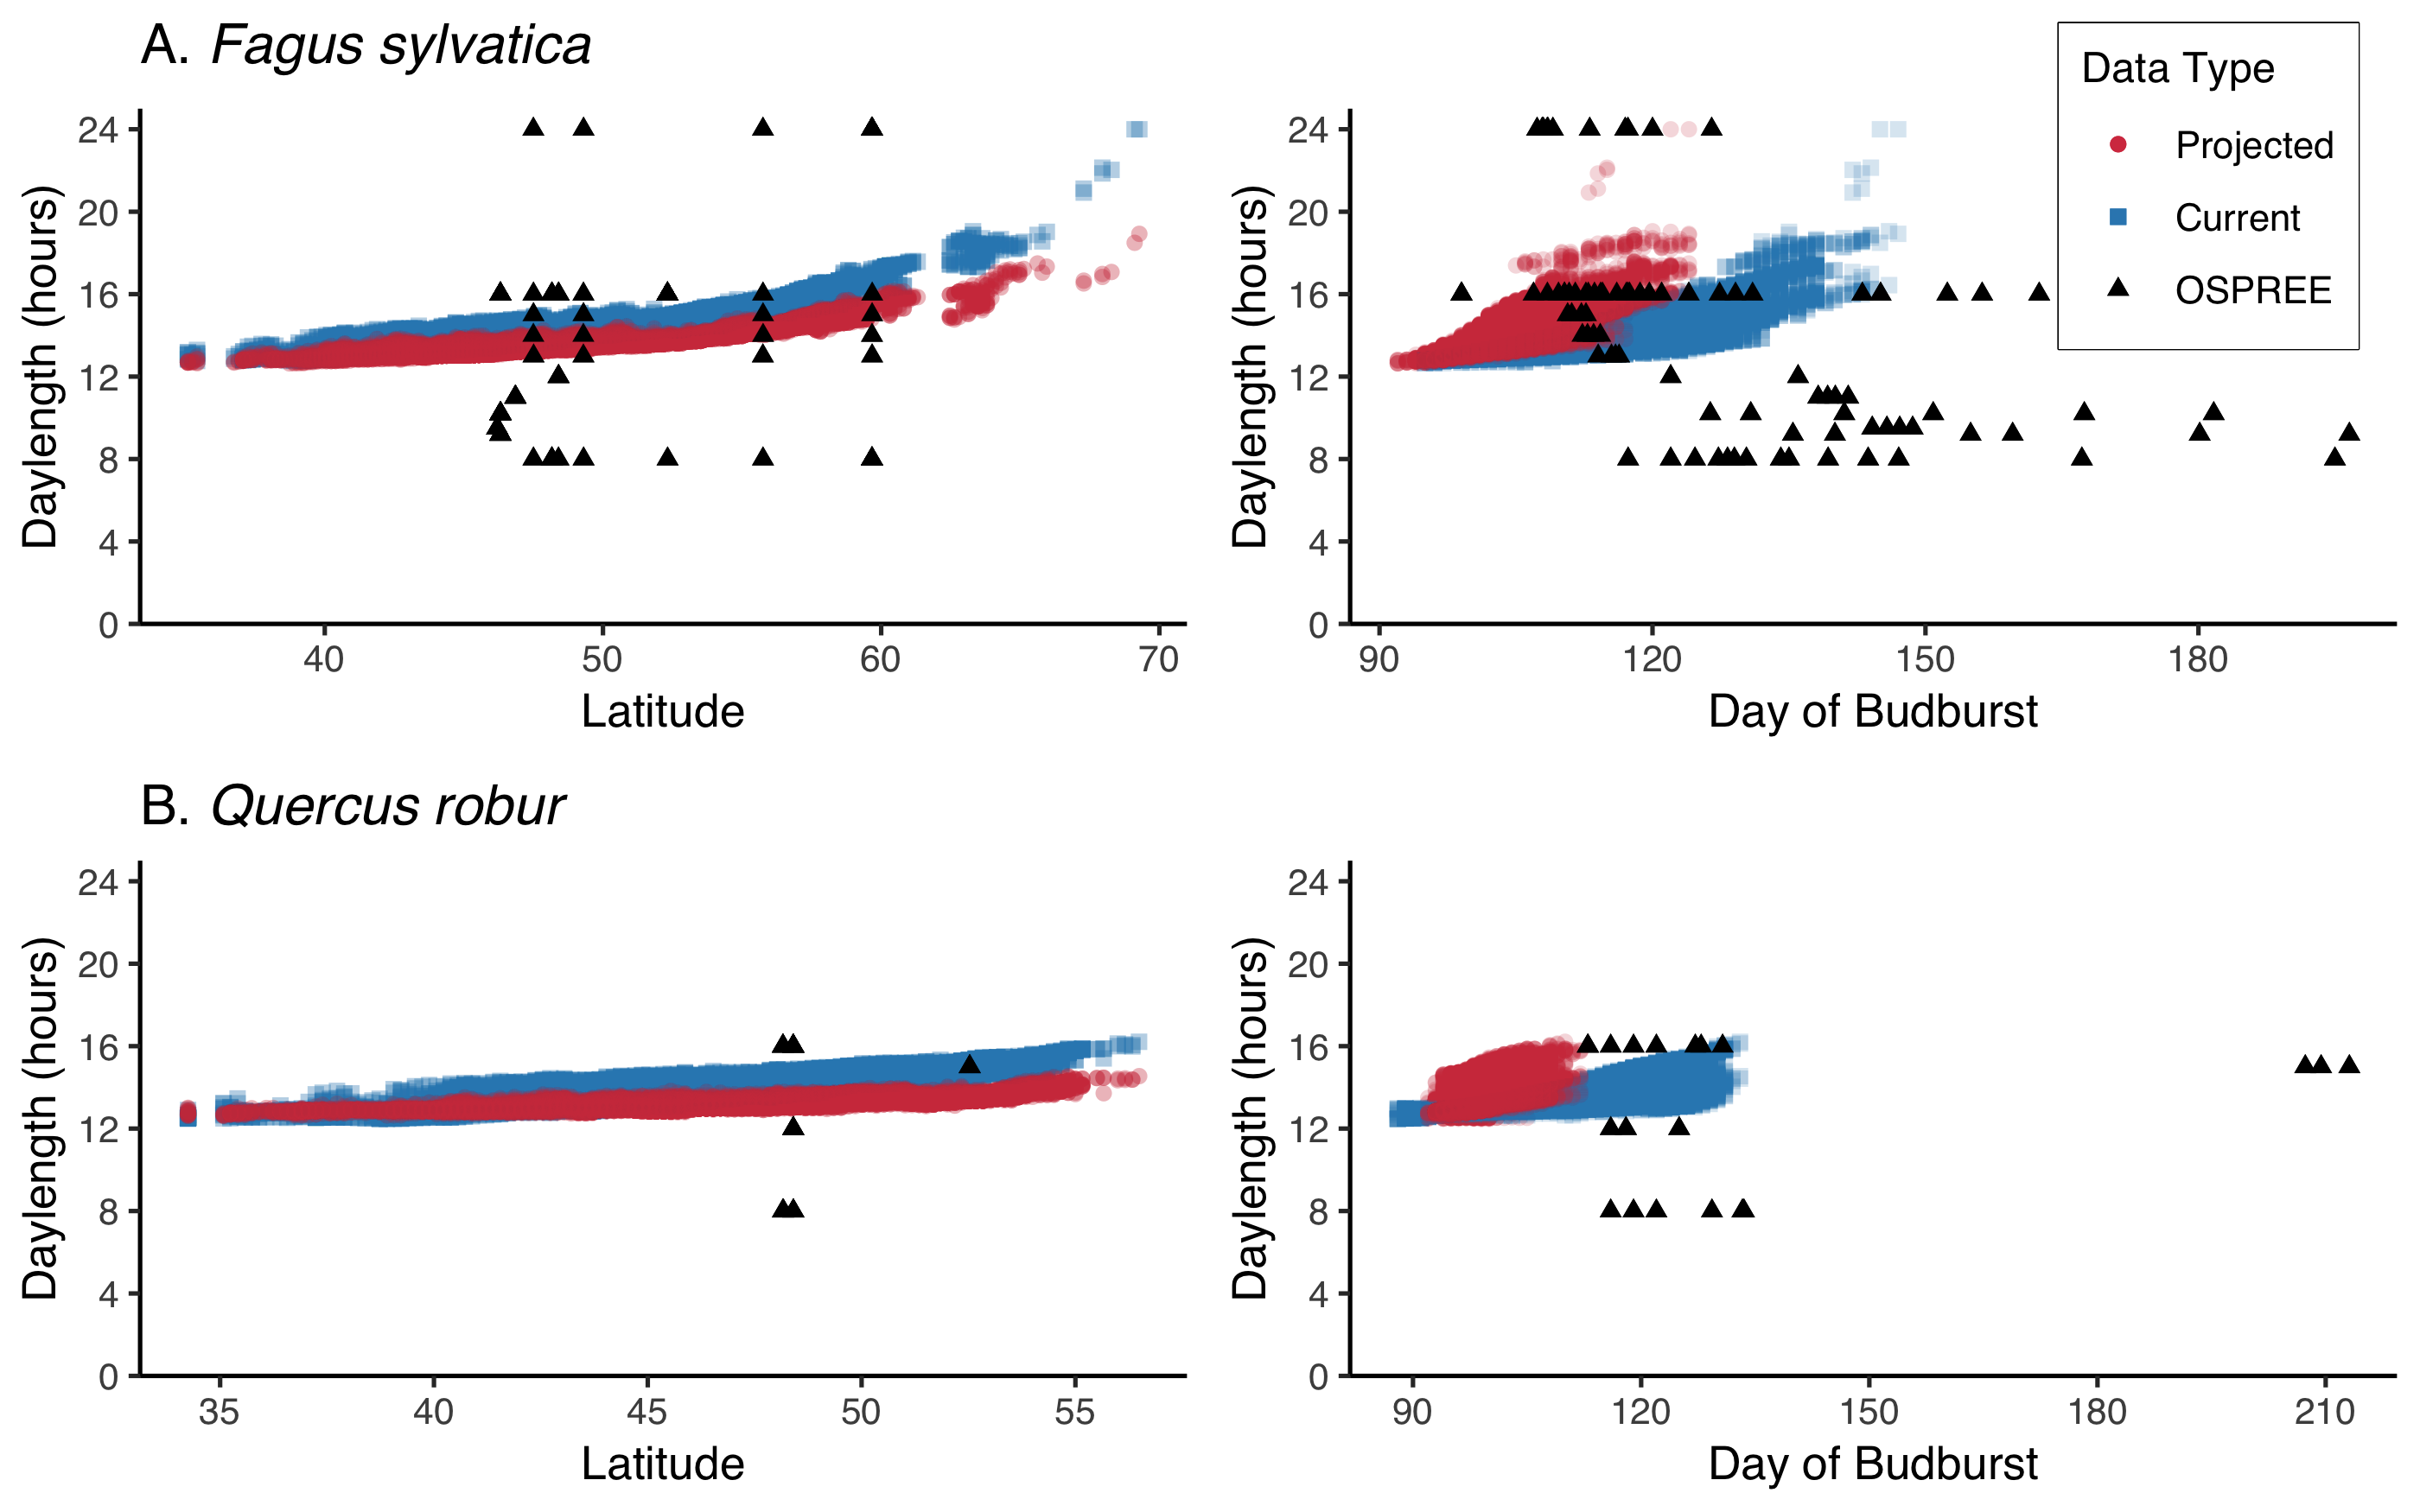
\includegraphics{/Users/aileneettinger/Documents/GitHub/ospree/analyses/photoperiod/figures/2D_actual_combined.png} 
\caption{\textbf{Experimental treatments of daylength in the OSPREE database} for \textit{Fagus sylvatica} (A) and \textit{Quercus robur} (B). For comparison, we show the daylength when budburst occurs in its current and projected ranges (left panels) and in its current range only, with expected shifts in phenology (right panels). Estimates and projections are from Phenofit \citep{duputie2015}}
 \label{fig:fagus}
 \end{figure}
 
\begin{figure}[p]
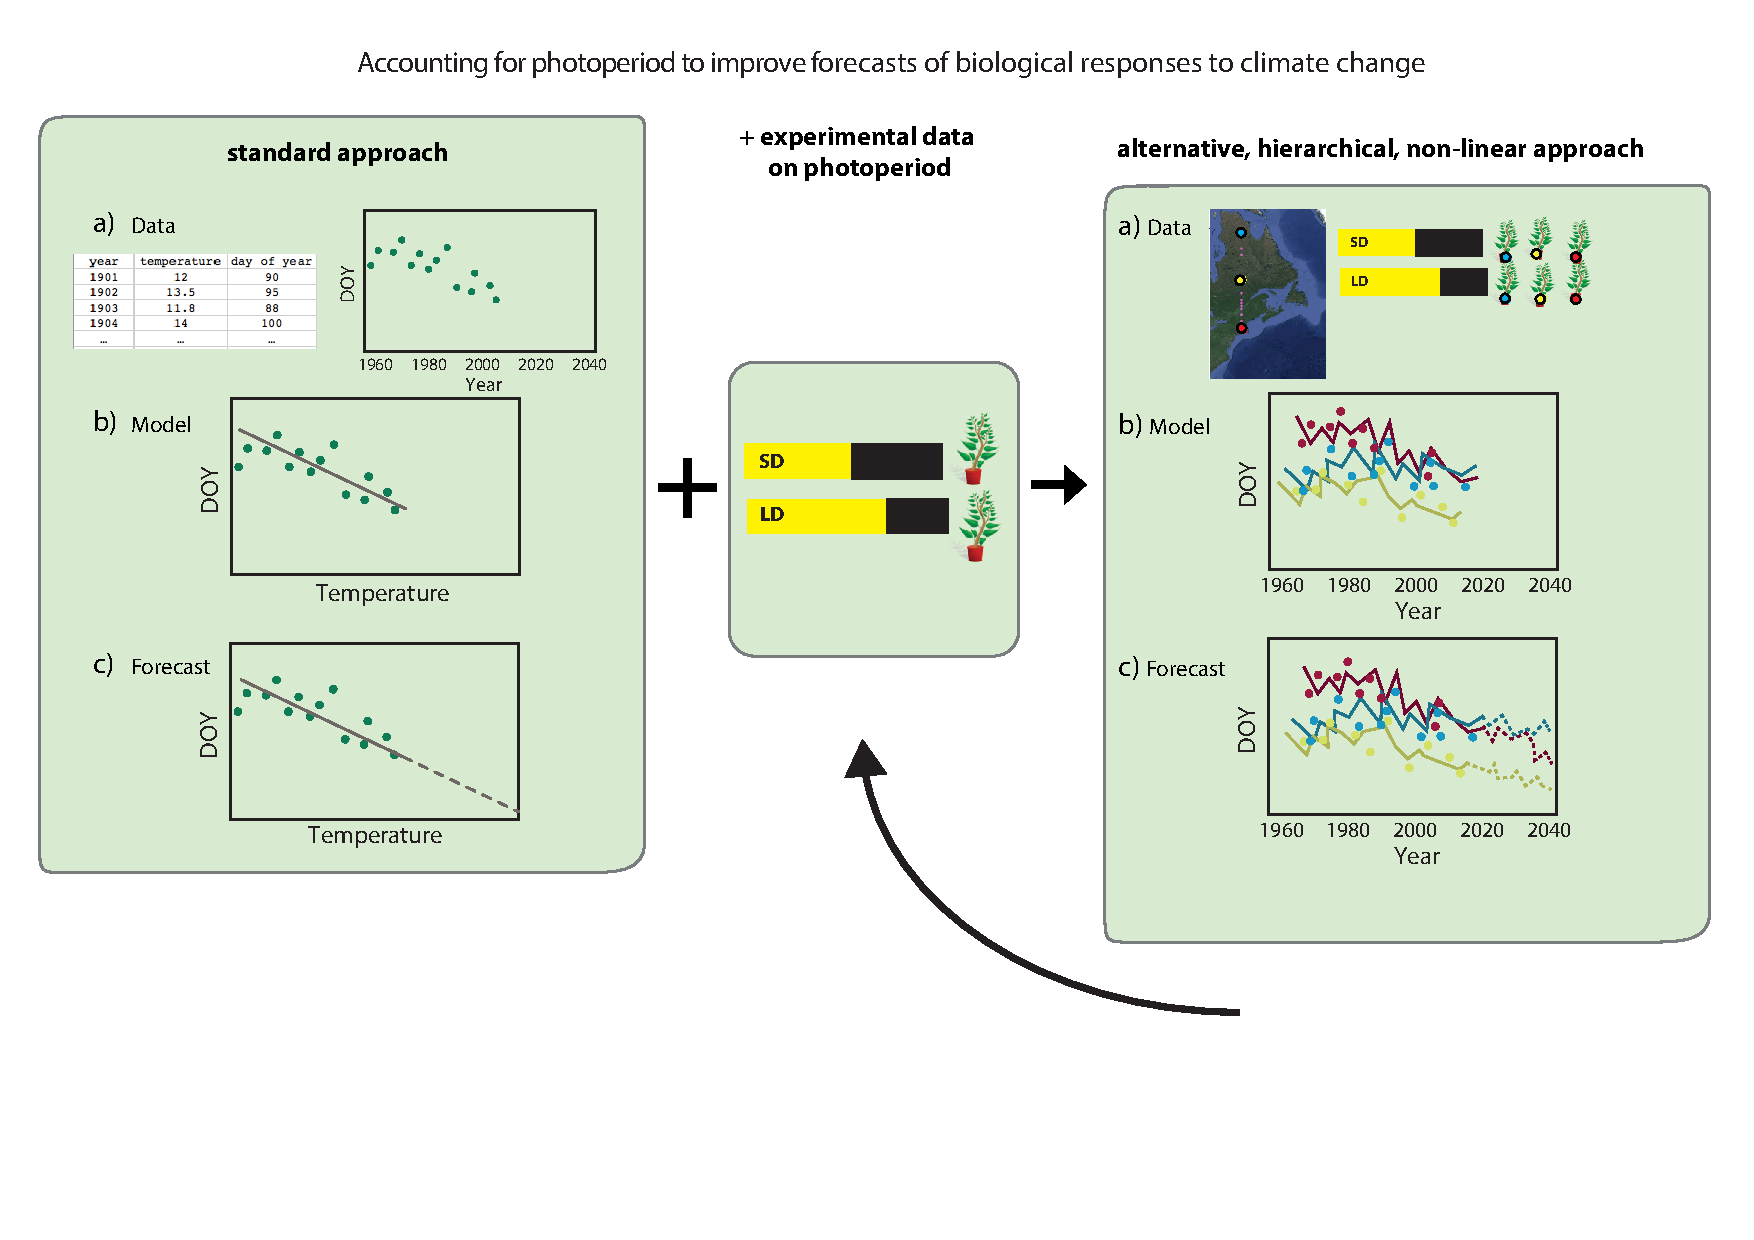
\includegraphics{/Users/aileneettinger/Documents/GitHub/ospree/analyses/photoperiod/figures/photocondiag4_AE.pdf} 
\caption{\textbf{Conceptual diagram of how to include photoperiod in forecasting biological responses to climate change}.}
 \label{fig:condiag}
 \end{figure}

%%%%%%%%%%%%%%%%%%%%%%%%%%%%%%%%%%%%%%%%
\end{document}
%%%%%%%%%%%%%%%%%%%%%%%%%%%%%%%%%%%%%%%%
